\chapter{Platform}
Redis is written in ANSI C and works in most POSIX systems like Linux, *BSD, OS X without external dependencies. Linux and OS X are the two operating systems where Redis is developed and more tested, and we recommend using Linux for deploying. Redis may work in Solaris-derived systems like SmartOS, but the support is best effort. There is no official support for Windows builds, but Microsoft develops and maintains a Win-64 port of Redis.

\section{Run Redis on Google Cloud Platform}
Redis is an open source (BSD licensed), in-memory data structure store, used as database, cache and message broker.
It's easy to get started developing Redis apps running on Google Cloud Platform. And because the apps you create will be running on the same infrastructure that powers all of Google's products, you can be confident that they will scale to serve all of your users, whether there are a few or millions of them.

The following diagram shows the process of deploying the app on Cloud Platform.

\begin{figure}[htb!]
	\centerline{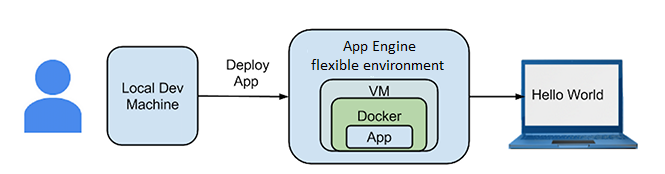
\includegraphics{resources/hello-world-app-structure.png}}
	\caption{Hello World App Structure}
	\label{hello-world-app-structure}
\end{figure}
The App Engine flexible environment runs your application in containers that can automatically scale to handle your application's load. Behind the scenes, this architecture uses both Compute Engine and Docker.